\documentclass[10pt]{article}
\usepackage[letterpaper]{geometry}
\geometry{verbose,tmargin=1in,bmargin=1in,lmargin=1in,rmargin=1in}
\usepackage{setspace}
\usepackage{ragged2e}
\usepackage{color}
\usepackage{titlesec}
\usepackage{graphicx}
\usepackage{float}
\usepackage{mathtools}
\usepackage{amsmath}
\usepackage[font=small,labelfont=bf,labelsep=period]{caption}
\usepackage[english]{babel}
\usepackage{indentfirst}
\usepackage{array}
\usepackage{makecell}
\usepackage[usenames,dvipsnames]{xcolor}
\usepackage{multirow}
\usepackage{tabularx}
\usepackage{arydshln}
\usepackage{caption}
\usepackage{subcaption}
\usepackage{xfrac}
\usepackage{etoolbox}
\usepackage{cite}
\usepackage{url}
\usepackage{dcolumn}
\usepackage{hyperref}
\usepackage{courier}
\usepackage{url}
\usepackage{esvect}
\usepackage{commath}
\usepackage{verbatim} % for block comments
\usepackage{enumitem}
\usepackage{hyperref} % for clickable table of contents
\usepackage{braket}
\usepackage{titlesec}
\usepackage{booktabs}
\usepackage{gensymb}
\usepackage{longtable}
\usepackage{listings}
\usepackage{cancel}
\usepackage{tcolorbox}
\usepackage[mathscr]{euscript}
\lstset{
    frame=single,
    breaklines=true,
    postbreak=\raisebox{0ex}[0ex][0ex]{\ensuremath{\color{red}\hookrightarrow\space}}
}

% for circled numbers
\usepackage{tikz}
\newcommand*\circled[1]{\tikz[baseline=(char.base)]{
            \node[shape=circle,draw,inner sep=2pt] (char) {#1};}}


\titleclass{\subsubsubsection}{straight}[\subsection]

% define new command for triple sub sections
\newcounter{subsubsubsection}[subsubsection]
\renewcommand\thesubsubsubsection{\thesubsubsection.\arabic{subsubsubsection}}
\renewcommand\theparagraph{\thesubsubsubsection.\arabic{paragraph}} % optional; useful if paragraphs are to be numbered

\titleformat{\subsubsubsection}
  {\normalfont\normalsize\bfseries}{\thesubsubsubsection}{1em}{}
\titlespacing*{\subsubsubsection}
{0pt}{3.25ex plus 1ex minus .2ex}{1.5ex plus .2ex}

\makeatletter
\renewcommand\paragraph{\@startsection{paragraph}{5}{\z@}%
  {3.25ex \@plus1ex \@minus.2ex}%
  {-1em}%
  {\normalfont\normalsize\bfseries}}
\renewcommand\subparagraph{\@startsection{subparagraph}{6}{\parindent}%
  {3.25ex \@plus1ex \@minus .2ex}%
  {-1em}%
  {\normalfont\normalsize\bfseries}}
\def\toclevel@subsubsubsection{4}
\def\toclevel@paragraph{5}
\def\toclevel@paragraph{6}
\def\l@subsubsubsection{\@dottedtocline{4}{7em}{4em}}
\def\l@paragraph{\@dottedtocline{5}{10em}{5em}}
\def\l@subparagraph{\@dottedtocline{6}{14em}{6em}}
\makeatother

\newcommand{\volume}{\mathop{\ooalign{\hfil$V$\hfil\cr\kern0.08em--\hfil\cr}}\nolimits}

\setcounter{secnumdepth}{4}
\setcounter{tocdepth}{4}
\begin{document}

\title{MATH 228b: HW1}
\author{April Novak}

\maketitle

\section{}

Transfinite Interpolation (TFI) is used to map from a master domain (defined in 2-D over \(0\leq\xi\leq1\) and \(0\leq\eta\leq1\)) to the physical domain by expressing the boundary of the physical domain in terms of \(\xi,\eta\) coordinates. This then constrains the master grid to lie within the physical domain boundaries. TFI does not guarantee a one-to-one mapping or orthogonality of the mesh, however, but is useful for directly controlling the grid spacing in a computationally efficient and easy manner. The mapping from the master domain to the physical domain is given by \(\textbf{X}(\xi,\eta)\):

\begin{equation}
\textbf{X}(\xi,\eta)=\left\lbrack x(\xi,\eta), y(\xi,\eta)\right\rbrack^T
\end{equation}

where \(x(\xi,\eta)\) and \(y(\xi,\eta)\) are the mappings from the individual coordinates in the master domain (\(\xi,\eta\)) to those in the physical domain (\(x,y\)). For \textit{linear} TFI, we construct 1-D, \textit{linear} interpolants in the \(x\) and \(y\) directions:

\begin{equation}
\begin{aligned}
\textbf{U}(\xi,\eta)=& (1-\xi_i)\textbf{X}(0,\eta_j)+\xi_i\textbf{X}(1,\eta_j)\\
\textbf{V}(\xi,\eta)=& (1-\eta_j)\textbf{X}(\xi_i,0)+\eta_j\textbf{X}(\xi_i,1)\\
\end{aligned}
\end{equation}

where \(\textbf{U}\) is the 1-D interpolant in the \(x\)-direction and \(\textbf{V}\) the 1-D interpolant in the \(y\)-direction. For a 2-D domain, \(x\) and \(y\) are functions of \(\xi\) and \(\eta\). The 2-D interpolant is constructed from the 1-D interpolants above by performing a Boolean sum.

\begin{equation}
\begin{aligned}
\textbf{X}(\xi,\eta)=& (1-\xi_i)\textbf{X}(0,\eta_j)+\xi_i\textbf{X}(1,\eta_j) + (1-\eta_j)\textbf{X}(\xi_i,0)+\eta_j\textbf{X}(\xi_i,1) - \\
& \left\lbrack(1-\xi_i)(1-\eta_j)\textbf{X}(0,0)+(1-\xi_i)\eta_j\textbf{X}(0,1)+\xi_i(1-\eta_j)\textbf{X}(1,0)+\xi_i\eta_j\textbf{X}(1,1)\right\rbrack
\end{aligned}
\end{equation}

The \(\textbf{X}\) that appear on the right-hand side of the equation above are assumed to be known, and is how the physical domain boundary enters the meshing algorithm. For a straight-sided domain, with corner coordinates \((x_1,y_1), (x_2,y_2), (x_3,y_3), (x_4, y_4)\), where the first coordinate pair is in the lower left corner, the interpolation along the sides is given by:

\begin{equation}
\begin{aligned}
\textbf{X}(0,\eta_j)=\begin{bmatrix}(1-\eta_j)x_1+\eta x_4\\ (1-\eta_j)y_0+\eta y_4\end{bmatrix}\\
\textbf{X}(1,\eta_j)=\begin{bmatrix}(1-\eta_j)x_2+\eta x_3\\ (1-\eta_j)y_2+\eta y_3\end{bmatrix}\\
\textbf{X}(\xi_i,0)=\begin{bmatrix}(1-\xi_i)x_1+\xi_i x_2\\ (1-\xi_i)y_1+\xi_i y_2\end{bmatrix}\\
\textbf{X}(\xi_i,1)=\begin{bmatrix}(1-\xi_i)x_4+\xi_i x_3\\ (1-\xi_i)y_4+\xi_i y_3\end{bmatrix}\\
\end{aligned}
\end{equation}

where a 2-D domain is used for simplicity - the results would equally extend to 3-D. Then, inserting these into the Boolean sum above gives:

\begin{equation}
\begin{aligned}
x(\xi,\eta)=& (1-\xi_i)\left((1-\eta_j)x_1+\eta_j x_4\right)+\xi_i\left((1-\eta_j)x_2+\eta x_3\right) + \\
&(1-\eta_j)\left((1-\xi_i)x_1+\xi_i x_2\right)+\eta_j\left((1-\xi_i)x_4+\xi_i x_3\right) - \\
& \left\lbrack(1-\xi_i)(1-\eta_j)x_1+(1-\xi_i)\eta_jx_4+\xi_i(1-\eta_j)x_2+\xi_i\eta_jx_3\right\rbrack\\
=& \cancel{(1-\xi_i)(1-\eta_j)x_1}+\cancel{(1-\xi_i)\eta_j x_4}+\cancel{\xi_i(1-\eta_j)x_2}+\cancel{\eta_j x_3\xi_i} +\\
&(1-\eta_j)(1-\xi_i)x_1+\xi_i x_2(1-\eta_j)+\eta_j(1-\xi_i)x_4+\xi_i x_3\eta_j-\\
& \left\lbrack\cancel{(1-\xi_i)(1-\eta_j)x_1}+\cancel{(1-\xi_i)\eta_jx_4}+\cancel{\xi_i(1-\eta_j)x_2}+\cancel{\xi_i\eta_jx_3}\right\rbrack\\
=& (1-\eta_j)(1-\xi_i)x_1+\xi_i x_2(1-\eta_j)+\eta_j(1-\xi_i)x_4+x_3\eta_j\xi_i\\
\end{aligned}
\end{equation}

From the last line above, it is seen that, for the transformation from \(\xi\) to \(x\), the linear TFI is equivalent to bilinear interpolation between the four corner points. Similarly, bilinear interpolation between the \(y\)-coordinates of the four corner points is also equivalent to a bilinear interpolation (work follows the same steps shown above).

\begin{equation}
\begin{aligned}
y(\xi,\eta)= (1-\eta_j)(1-\xi_i)y_1+\xi_i y_2(1-\eta_j)+\eta_j(1-\xi_i)y_4+ y_3\eta_j\xi_i\\
\end{aligned}
\end{equation}

\section{}

TFI is used to generate a structured mesh of the given domain. The 1-D interpolations in the \(x\) and \(y\) directions now include four terms, two to account for control of the 1-D boundary values, and two to control for the 1-D boundary derivatives.

\begin{equation}
\begin{aligned}
\textbf{U}(\xi,\eta)=(2\xi_i^3-3\xi_i^2+1)\textbf{X}(0,\eta_j)+(3\xi_i^2-2\xi_i^3)\textbf{X}(1,\eta_j)+(\xi_i^3-2\xi_i^2+\xi_i)\frac{\partial\textbf{X}(0,\eta_j)}{\partial\xi}+(\xi_i^3-\xi_i^2)\frac{\partial\textbf{X}(1,\eta_j)}{\partial\xi}\\
\textbf{V}(\xi,\eta)=(2\eta_j^3-3\eta_j^2+1)\textbf{X}(\xi_i,0)+(3\eta_j^2-2\eta_j^3)\textbf{X}(\xi_i,1)+(\eta_j^3-2\eta_j^2+\eta_j)\frac{\partial\textbf{X}(\xi_i,0)}{\partial\eta}+(\eta_j^3-\eta_j^2)\frac{\partial\textbf{X}(\xi_i,1)}{\partial\eta}\\
\end{aligned}
\end{equation}

The 2-D interpolant is constructed from the 1-D interpolants by performing a Boolean sum:

\begin{equation}
\begin{aligned}
\textbf{X}(\xi,\eta)=& (2\xi_i^3-3\xi_i^2+1)\textbf{X}(0,\eta_j)+(3\xi_i^2-2\xi_i^3)\textbf{X}(1,\eta_j)+(\xi_i^3-2\xi_i^2+\xi_i)\frac{\partial\textbf{X}(0,\eta_j)}{\partial\xi}+(\xi_i^3-\xi_i^2)\frac{\partial\textbf{X}(1,\eta_j)}{\partial\xi}+\\
& (2\eta_j^3-3\eta_j^2+1)\textbf{X}(\xi_i,0)+(3\eta_j^2-2\eta_j^3)\textbf{X}(\xi_i,1)+(\eta_j^3-2\eta_j^2+\eta_j)\frac{\partial\textbf{X}(\xi_i,0)}{\partial\eta}+(\eta_j^3-\eta_j^2)\frac{\partial\textbf{X}(\xi_i,1)}{\partial\eta}-\\
& \left\lbrack(2\xi_i^3-3\xi_i^2+1)(2\eta_j^3-3\eta_j^2+1)\textbf{X}(0,0)+(2\xi_i^3-3\xi_i^2+1)(3\eta_j^2-2\eta_j^3)\textbf{X}(0,1)\right\rbrack-\\
& \left\lbrack(2\xi_i^3-3\xi_i^2+1)(\eta_j^3-2\eta_j^2+\eta_j)\frac{\partial\textbf{X}(0,0)}{\partial\eta}+(2\xi_i^3-3\xi_i^2+1)(\eta_j^3-\eta_j^2)\frac{\partial\textbf{X}(0,1)}{\partial\eta}\right\rbrack-\\
& \left\lbrack(3\xi_i^2-2\xi_i^3)(2\eta_j^3-3\eta_j^2+1)\textbf{X}(1,0)+(3\xi_i^2-2\xi_i^3)(3\eta_j^2-2\eta_j^3)\textbf{X}(1,1)\right\rbrack-\\
& \left\lbrack(3\xi_i^2-2\xi_i^3)(\eta_j^3-2\eta_j^2+\eta_j)\frac{\partial\textbf{X}(1,0)}{\partial\eta}+(3\xi_i^2-2\xi_i^3)(\eta_j^3-\eta_j^2)\frac{\partial\textbf{X}(1,1)}{\partial\eta}\right\rbrack-\\
& \left\lbrack(\xi_i^3-2\xi_i^2+1)(2\eta_j^3-3\eta_j^2+1)\frac{\partial\textbf{X}(0,0)}{\partial\xi}+(\xi_i^3-2\xi_i^2+\xi_i)(3\eta_j^2-2\eta_j^3)\frac{\partial\textbf{X}(0,1)}{\partial\xi}\right\rbrack-\\
& \left\lbrack(\xi_i^3-2\xi_i^2+1)(\eta_j^3-2\eta_j^2+\eta_j)\frac{\partial\textbf{X}(0,0)}{\partial\xi\partial\eta}+(\xi_i^3-2\xi_i^2+\xi_i)(\eta_j^3-\eta_j^2)\frac{\partial\textbf{X}(0,1)}{\partial\xi\partial\eta}\right\rbrack-\\
& \left\lbrack(\xi_i^3-\xi_i^2)(2\eta_j^3-3\eta_j^2+1)\frac{\partial\textbf{X}(1,0)}{\partial\xi}+(\xi_i^3-\xi_i^2)(3\eta_j^2-2\eta_j^3)\frac{\partial\textbf{X}(1,1)}{\partial\xi}\right\rbrack-\\
& \left\lbrack(\xi_i^3-\xi_i^2)(\eta_j^3-2\eta_j^2+\eta_j)\frac{\partial\textbf{X}(1,0)}{\partial\xi\partial\eta}+(\xi_i^3-\xi_i^2)(\eta_j^3-\eta_j^2)\frac{\partial\textbf{X}(1,1)}{\partial\xi\partial\eta}\right\rbrack
\end{aligned}
\end{equation}

For the given domain, the \textbf{X} functions along the sides are given by:

\begin{equation}
\begin{aligned}
\textbf{X}(\xi, 0)=& \left\lbrack\xi, (1-cos(2\pi\xi))/5\right\rbrack^T\\
\textbf{X}(\xi, 1)=& \left\lbrack\xi, 1+(1-cos(\pi \xi))/5\right\rbrack^T\\
\textbf{X}(0, \eta)=& \left\lbrack0, \eta\right\rbrack^T\\
\textbf{X}(1, \eta)=& \left\lbrack1, 1.4\eta\right\rbrack^T\\
\end{aligned}
\end{equation}

where the values at the corners are:

\begin{equation}
\begin{aligned}
\textbf{X}(0, 0)=& \left\lbrack0, 0\right\rbrack^T\\
\textbf{X}(0, 1)=& \left\lbrack0, 1\right\rbrack^T\\
\textbf{X}(1, 0)=& \left\lbrack1, 0\right\rbrack^T\\
\textbf{X}(1, 1)=& \left\lbrack1, 1.4\right\rbrack^T\\
\end{aligned}
\end{equation}

And the normals along the boundaries, to be used in the specification of the derivatives according to the problem statement, are:

\begin{equation}
\begin{aligned}
\hat{n}(\textrm{bottom side})=&\frac{\left\lbrack-2\pi sin(2\pi\xi)/5, 1\right\rbrack^T}{\sqrt{(-2\pi sin(2\pi\xi)/5)^2+1}}\\
\hat{n}(\textrm{top side})=&\frac{\left\lbrack-\pi sin(\pi\xi)/5, 1\right\rbrack^T}{\sqrt{(-\pi sin(\pi\xi)/5)^2+1}}\\
\hat{n}(\textrm{left side})=&\left\lbrack1, 0\right\rbrack^T\\
\hat{n}(\textrm{right side})=&\left\lbrack1, 0\right\rbrack^T\\
\end{aligned}
\end{equation}

Fig. \ref{fig:hermite} shows the mesh generated using \(T=0.5\). As can be seen, boundary orthogonality is achieved on all sides. For simplicity, the second derivative terms were all assumed to be zero, since they would be zero on the left and right edges, and all corners points can be expressed as either belonging to the right and left edges, or either to the top and bottom edges.

\begin{figure}[H]
\centering
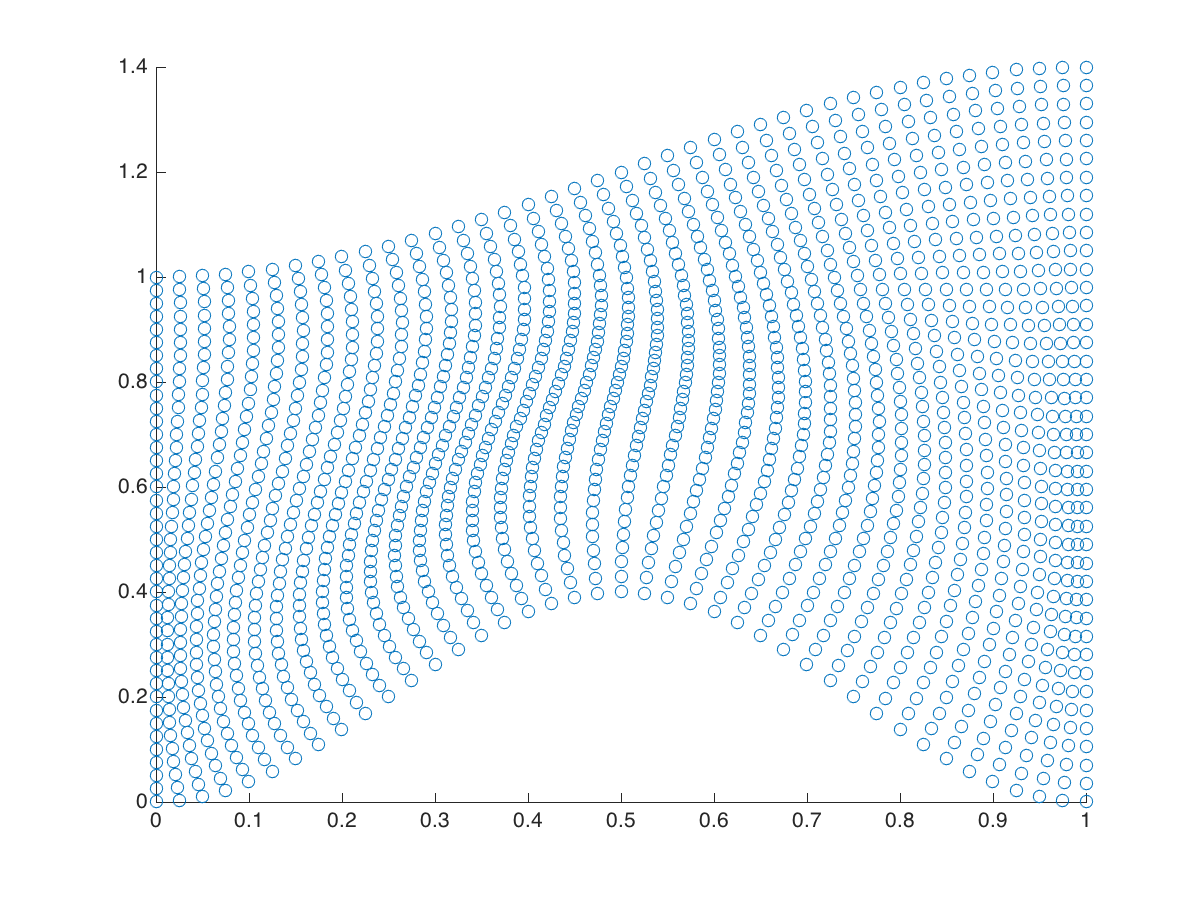
\includegraphics[width=0.5\textwidth]{hermite_plot.png}
\caption{Hermite mapping.}
\label{fig:hermite}
\end{figure}

\section{}

For a conformal map, an analytic function can be mapped to the domain \(w=u+iv\) for a variable \(z=x+iy\).

\begin{equation}
\begin{aligned}
w=&\frac{2e^z-3}{3e^z-2}\\
=& \frac{2e^{x+iy}-3}{3e^{x+iy}-2}\\
\end{aligned}
\end{equation}

Then, multiply this expression by the complex conjugate of the denominator to find how \(x,y\) maps to \(u,v\). 

\begin{equation}
\begin{aligned}
w=& \left(\frac{2e^{x+iy}-3}{3e^{x+iy}-2}\right)\left(\frac{3e^{x-iy}-2}{3e^{x-iy}-2}\right)\\
=& \frac{6e^{x+iy}e^{x-iy}-4e^{x+iy}-9e^{x-iy}+6}{9e^{x+iy}e^{x-iy}-6e^{x+iy}+-6e^{x-iy}+4}\\
=& \frac{6e^{2x}-13e^xcos(y)+5e^xisin(y)+6}{9e^{2x}-12e^xcos(y)+4}\\
=& \frac{6e^{2x}-13e^xcos(y)+6}{9e^{2x}-12e^xcos(y)+4}+i\frac{5e^xsin(y)}{9e^{2x}-12e^xcos(y)+4}\\
\end{aligned}
\end{equation}

\(x,y\) maps to \(u,v\) based on the following expressions.

\begin{equation}
\label{eq:Trans}
\begin{aligned}
u =& \frac{6e^{2x}-13e^xcos(y)+6}{9e^{2x}-12e^xcos(y)+4}\\
v =& \frac{5e^xsin(y)}{9e^{2x}-12e^xcos(y)+4}\\
\end{aligned}
\end{equation}

Fig. \ref{fig:q3} shows the mesh generated by uniformly discretizing \(x\) into 21 values and \(y\) into 81 values, and then using the above conformal mapping to determine the coordinates in the \(u, v\) coordinate system. The code written for this section is given in the Appendix.

\begin{figure}[H]
\centering
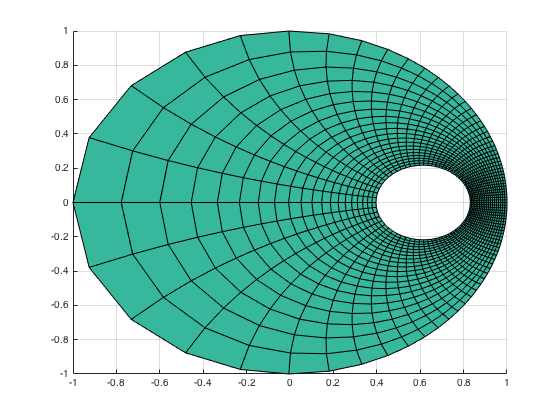
\includegraphics[width=0.5\textwidth]{Question3.png}
\caption{Conformal mapping structured mesh in the \(u, v\) coordinate system.}
\label{fig:q3}
\end{figure}

This transformation can also be shown by looking at the transformation values along the edges of the \(x,y\) domain by substituting in the appropriate values of \(x\) and \(y\) into Eq. \eqref{eq:Trans}. \(u\) transforms according to: 

\begin{equation}
\begin{aligned}
\textrm{Along left edge } (x=0, y=y): u=& \frac{12-13cos(y)}{13-12cos(y)}\\
\textrm{Along right edge } (x=1, y=y): u=& \frac{(6e^{2}+6)-13ecos(y)}{(9e^{2}+4)-12ecos(y)}\\
\textrm{Along bottom edge } (x=x, y=0): u=& \frac{6e^{2x}-13e^x+6}{9e^{2x}-12e^x+4}\\
\textrm{Along top edge } (x=x, y=2\pi): u=& \frac{6e^{2x}-13e^x+6}{9e^{2x}-12e^x+4}\\
\end{aligned}
\end{equation}

\(v\) transforms according to:

\begin{equation}
\begin{aligned}
\textrm{Along left edge } (x=0, y=y): v=& \frac{5sin(y)}{13-12cos(y)}\\
\textrm{Along right edge } (x=1, y=y): v=& \frac{5esin(y)}{(9e^{2}+4)-12ecos(y)}\\
\textrm{Along bottom edge } (x=x, y=0): v=& 0\\
\textrm{Along top edge } (x=x, y=2\pi): v=& 0\\
\end{aligned}
\end{equation}

Because \(u\) transforms the same way for the bottom and top edges, the bottom and top edges of the \(x,y\) domain ``touch'' in the \(u,v\) domain. Because \(0\leq x\leq1\), and \(v=0\) along the bottom and top edges, the bottom and top edges in the master domain map to the line segment between \(-1\leq u\leq (6e^2-13e+6)/(9e^2-12e+4)\approx 0.395\). 

The left side of the master domain gets mapped to the ``outside'' of the conformal map, while the right side of the physical domain is mapped to the perimeter of the inner circle. Along the left side of the master domain, \(x=0\) and \(y=y\), giving the following transformations:

\begin{equation}
\begin{aligned}
u=& \frac{12-13cos(y)}{13-12cos(y)}
v=& \frac{5sin(y)}{13-12cos(y)}\\
\end{aligned}
\end{equation}

For a circle, the general equation is \(u^2+v^2=r^2\), where \(r\) is the radius of the circle. By computing the left-hand side of this expression, it is shown that the outer boundary of the conformal map is a circle with radius \(1\), which is observed in the mesh shown above. With the \(0,0\) coordinate mapping to \(-1,0\) as given by the above expressions, this shows how the outer boundary of the conformal map is determined.

\begin{equation}
\begin{aligned}
u^2+v^2& =\frac{(12-13cos(y))^2}{(13-12cos(y))^2}+\frac{(5sin(y))^2}{(13-12cos(y))^2}\\
& =\frac{144-312cos(y)+169cos^2(y)+25sin^2(y)}{169-312cos(y)+144cos^2(y)}\\
& =\frac{144-312cos(y)+25(cos^2(y)+sin^2(y))+144cos^2(y)}{169-312cos(y)+144cos^2(y)}\\
& =\frac{169-312cos(y)+144cos^2(y)}{169-312cos(y)+144cos^2(y)}\\
& = 1\\
\end{aligned}
\end{equation}

For the inner circle, because \(v=0\) on the edge of the circle, the \(v\) coordinate is not offset from the origin, so the equation for this circle is given by:

\begin{equation}
(u-u_0)^2+v^2=r^2
\end{equation}

where \((u_0,0)\) is the center of the small circle. The diameter of the circle is given by the difference in \(u\) between the left edge of the circle (corresponding to the \((x=1,y=0)\) point in the master domain) and the right edge of the circle (corresponding to the \((x=1,y=\pi)\) point in the master domain). 

\begin{equation}
\label{eq:radius}
r=\frac{1}{2}\left(\frac{(6e^{2}+6)+13e}{(9e^{2}+4)+12e}-\frac{(6e^{2}+6)-13e}{(9e^{2}+4)-12e}\right)=\frac{5e}{9e^2-4}
\end{equation}

Hence, to show that the right edge maps to the inner circle, the equation for the circle is computed in order to find the radius above:

\begin{equation}
\left(\frac{6e^{2}+6-13ecos(y)}{9e^{2}+4-12ecos(y)}-\left(\frac{(6e^{2}+6)-13e}{(9e^{2}+4)-12e}+\frac{5e}{9e^2-4}\right)\right)^2+\left(\frac{5esin(y)}{b-12ecos(y)}\right)^2=r^2
\end{equation}

Because this algebra would be very messy, it is not carried out here, but performing the algebra above would show that \(r\) is indeed given by Eq. \eqref{eq:radius}, showing that the mapping does map the right edge to the inner circle.

\section{}

Delaunay triangulation is used to generate an unstructured, triangular mesh of the given polygonal domain. For a given maximum element size, the boundary is discretized such that each element has a length as close as possible to \(h_{max}\), but not exceeding this value. Then, the domain is triangulated using Delaunay triangulation. Triangles outside the domain are deleted by placing a point at the midpoint of each side of every triangle, and then testing to see if that point is outside the domain using the {\tt inpolygon} command. This is a relatively simple method of determining whether a line is outside the polygon, and will only work for relatively simple geometries. For instance, if only a portion of a line extends outside the domain, then this procedure might not work, since the midpoint of the line might be inside the domain, but the entire line may not be inside the domain. This would require a constrained Delaunay formulation, which is beyond the scope of this assignment. 

Triangles with a side outside the domain are deleted, and the triangulation process repeated until all triangles have a size no larger than \(h_{max}^2/2\). Triangles with areas larger than this maximum value are considered to be poor triangles from a mesh quality standpoint, and their circumcenter is added. This algorithm is not implemented in a very robust manner, however, since that circumcenter must be in the domain for the refinement process to continue to completion, since if the circumcenter is outside the domain, then that point is deleted, and an infinite loop is entered. So, this is a second reason why my implementation only works for relatively simple geometries. Once all triangles have an area smaller than the maximum allowable area, the mesh if refined uniformly \(n_{ref}\) times. For each refinement, the center of each mesh edge is added, and the triangulation performed to get a roughly twice-as-fine mesh as the previous uniform refinement level. For the polygon given, Fig. \ref{fig:original} shows the Delaunay triangulation obtained for (a) zero, (b) one, and (c) two uniform refinements for \(h_{max}=0.2\).

\begin{figure}[H]
        \centering
        \begin{subfigure}[b]{0.35\textwidth}
                \centering
                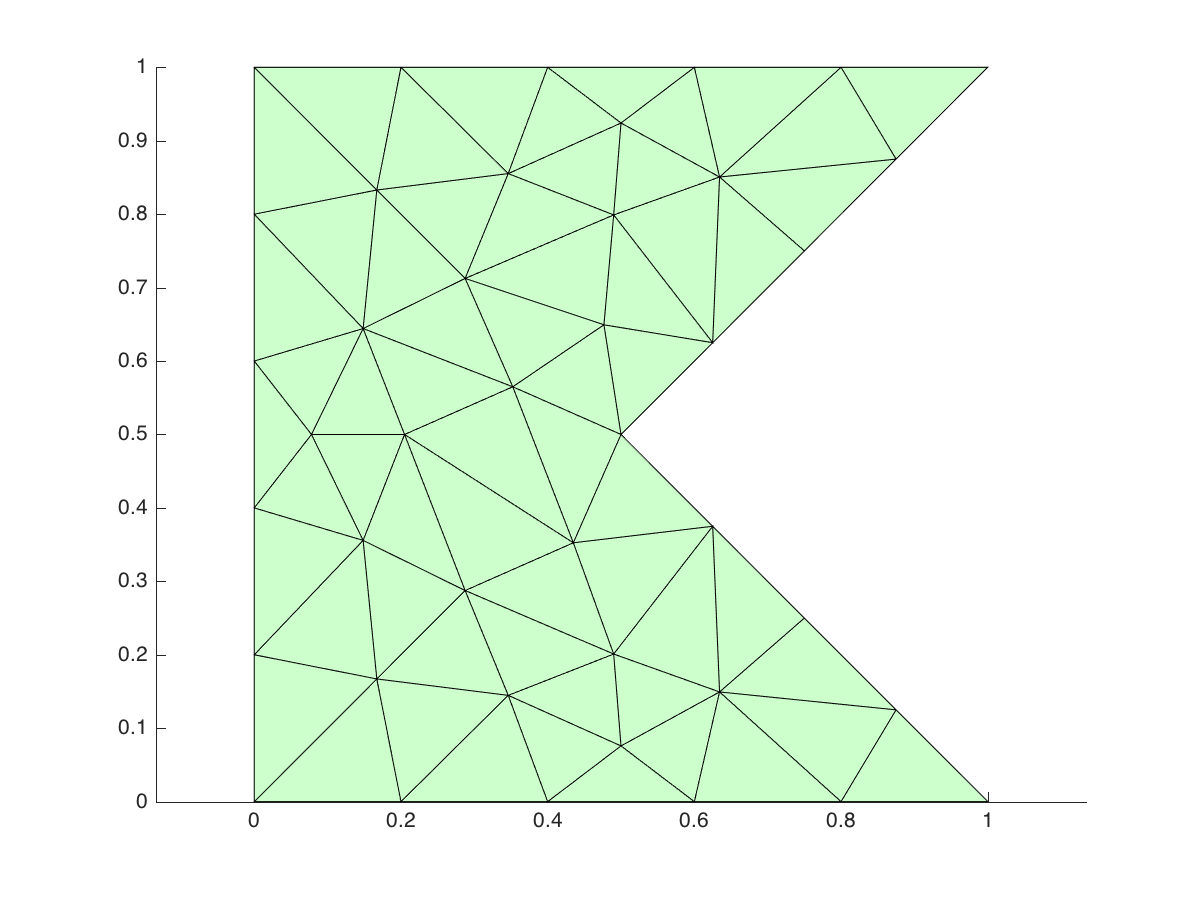
\includegraphics[width=\textwidth]{refine0.png}
                \caption{\(n_{ref}=0\)}
        \end{subfigure}%
        \begin{subfigure}[b]{0.35\textwidth}
                \centering
                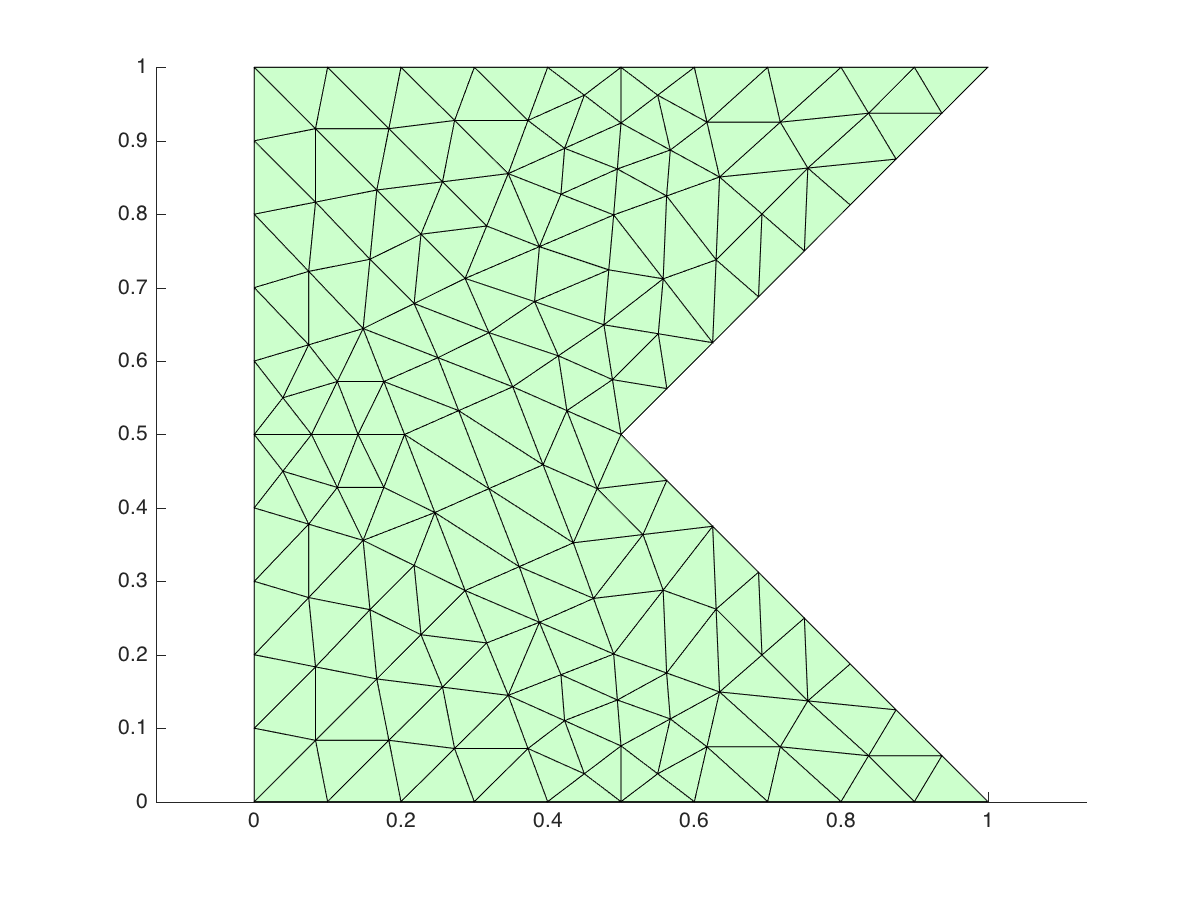
\includegraphics[width=\textwidth]{refine1.png}
                \caption{\(n_{ref}=1\)}
        \end{subfigure}%
        \begin{subfigure}[b]{0.35\textwidth}
                \centering
                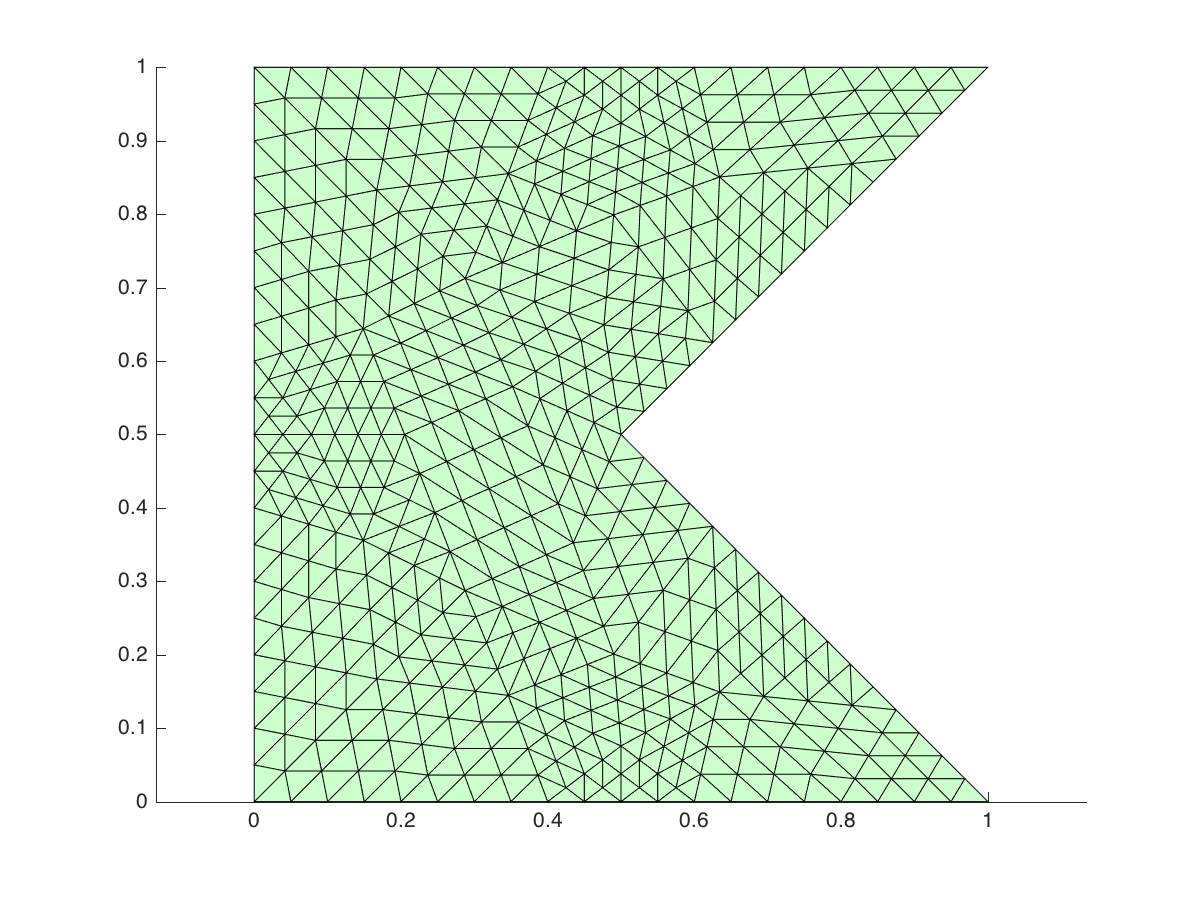
\includegraphics[width=\textwidth]{refine2.png}
                \caption{\(n_{ref}=2\)}
        \end{subfigure}%
        \caption{Uniform refinement for the starting polygon.}
        \label{fig:original}
\end{figure}

Two more examples of different polygons are shown in Figs. \ref{fig:stop} and \ref{fig:2}.

\begin{figure}[H]
        \centering
        \begin{subfigure}[b]{0.35\textwidth}
                \centering
                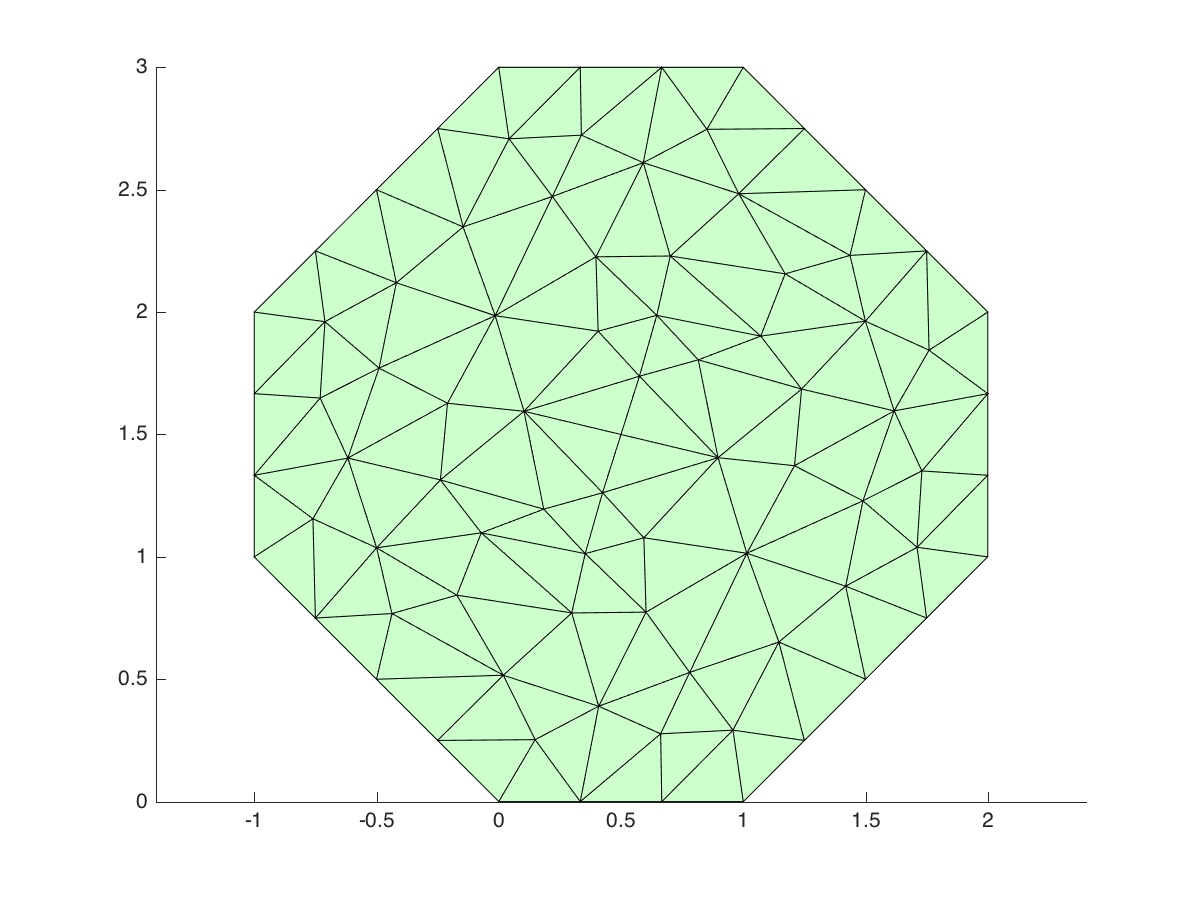
\includegraphics[width=\textwidth]{refine-A0.png}
                \caption{\(n_{ref}=0\)}
        \end{subfigure}%
        \begin{subfigure}[b]{0.35\textwidth}
                \centering
                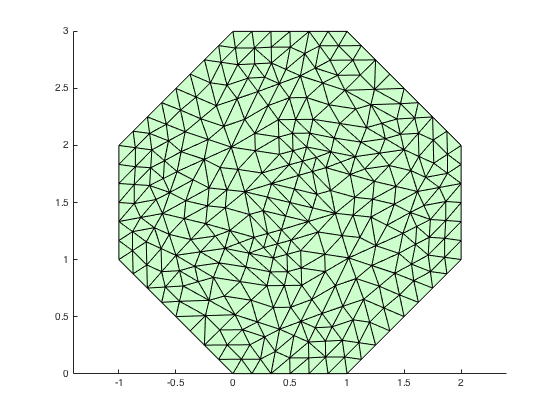
\includegraphics[width=\textwidth]{refine-A1.png}
                \caption{\(n_{ref}=1\)}
        \end{subfigure}%
        \begin{subfigure}[b]{0.35\textwidth}
                \centering
                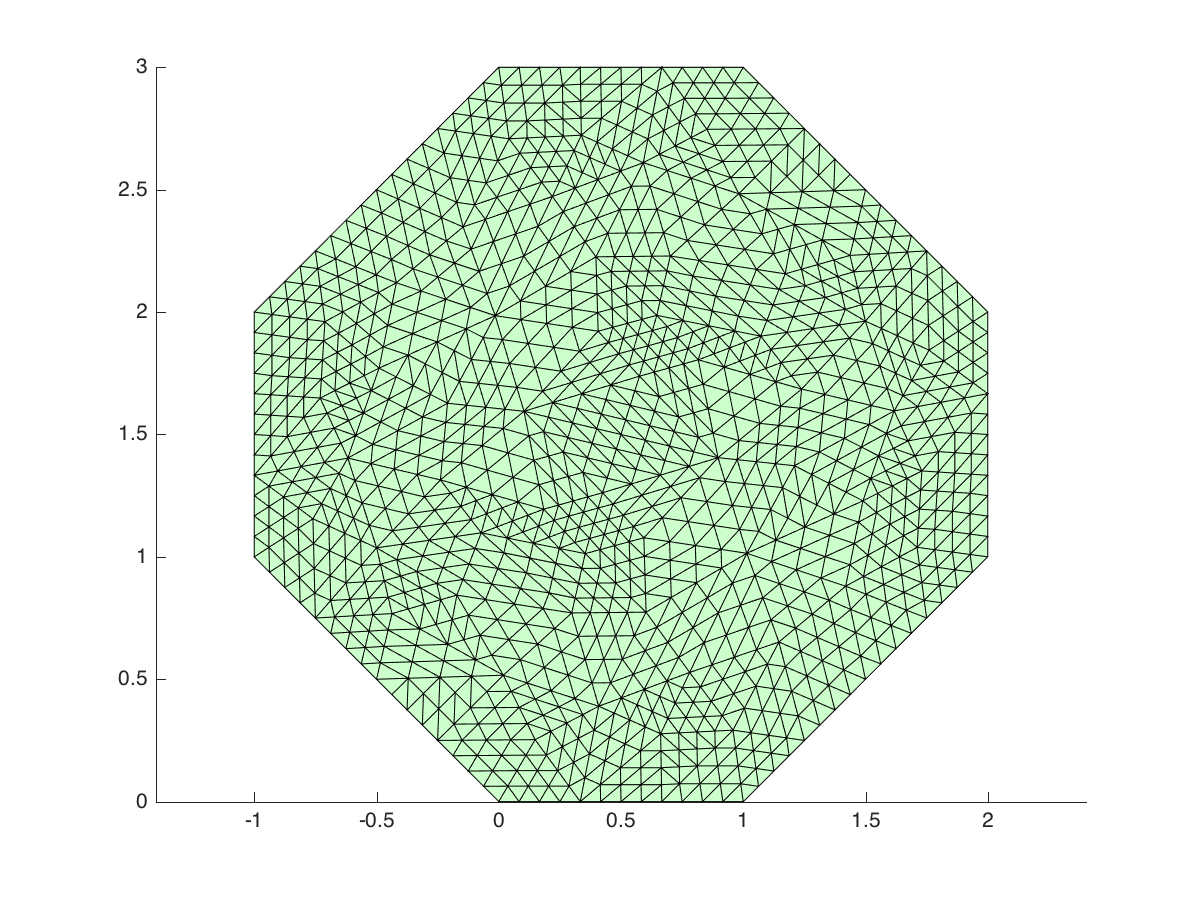
\includegraphics[width=\textwidth]{refine-A2.png}
                \caption{\(n_{ref}=2\)}
        \end{subfigure}%
        \caption{Uniform refinement for different polygon, for \(h_{max}=4\).}
        \label{fig:stop}
\end{figure}

\begin{figure}[H]
        \centering
        \begin{subfigure}[b]{0.35\textwidth}
                \centering
                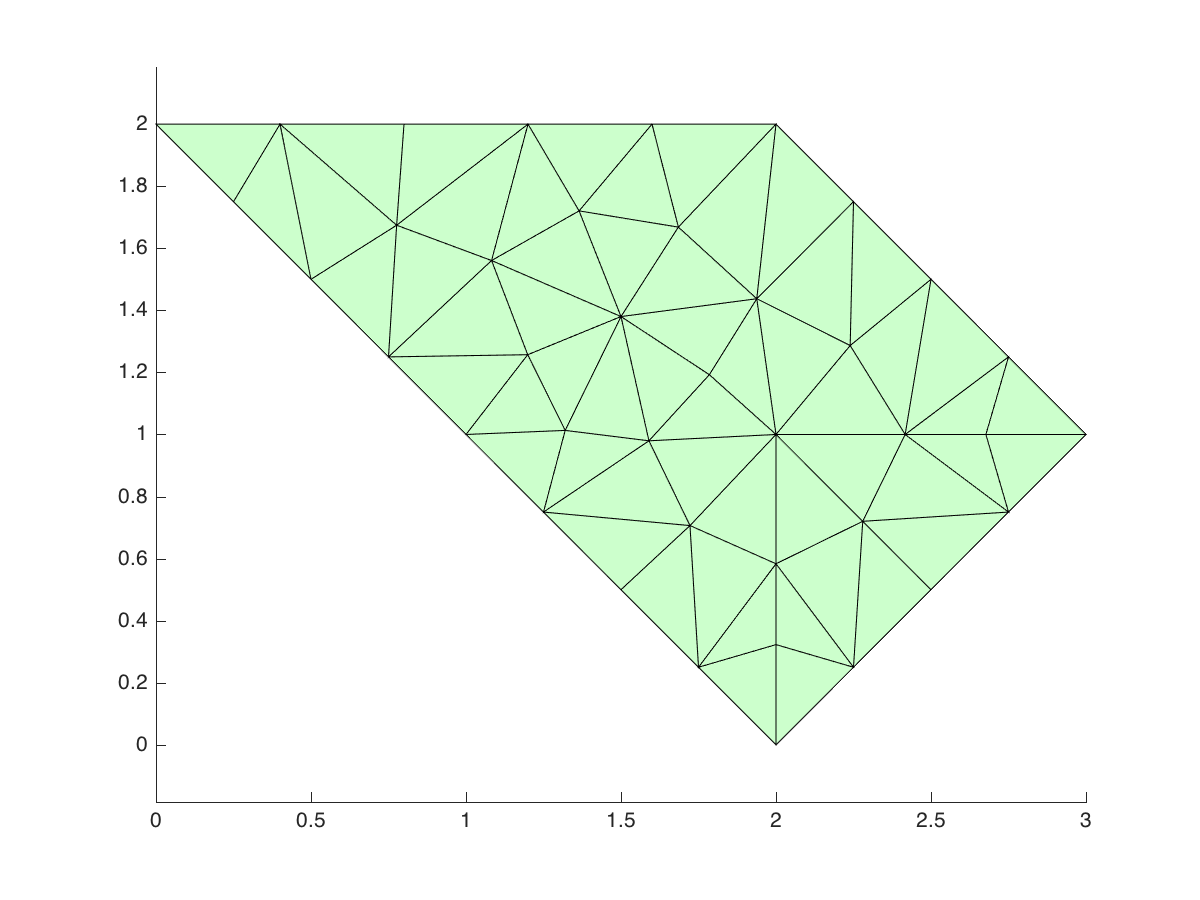
\includegraphics[width=\textwidth]{refine-B0.png}
                \caption{\(n_{ref}=0\)}
        \end{subfigure}%
        \begin{subfigure}[b]{0.35\textwidth}
                \centering
                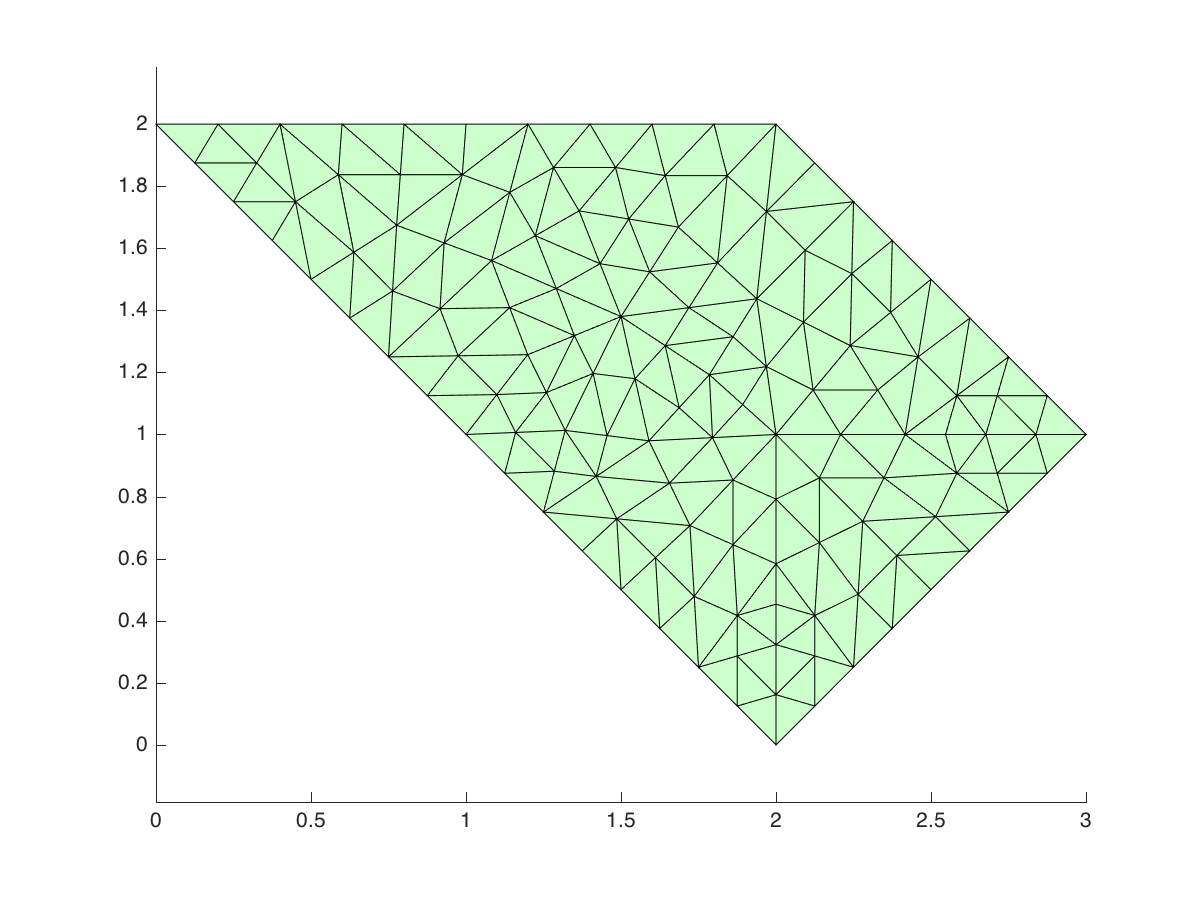
\includegraphics[width=\textwidth]{refine-B1.png}
                \caption{\(n_{ref}=1\)}
        \end{subfigure}%
        \begin{subfigure}[b]{0.35\textwidth}
                \centering
                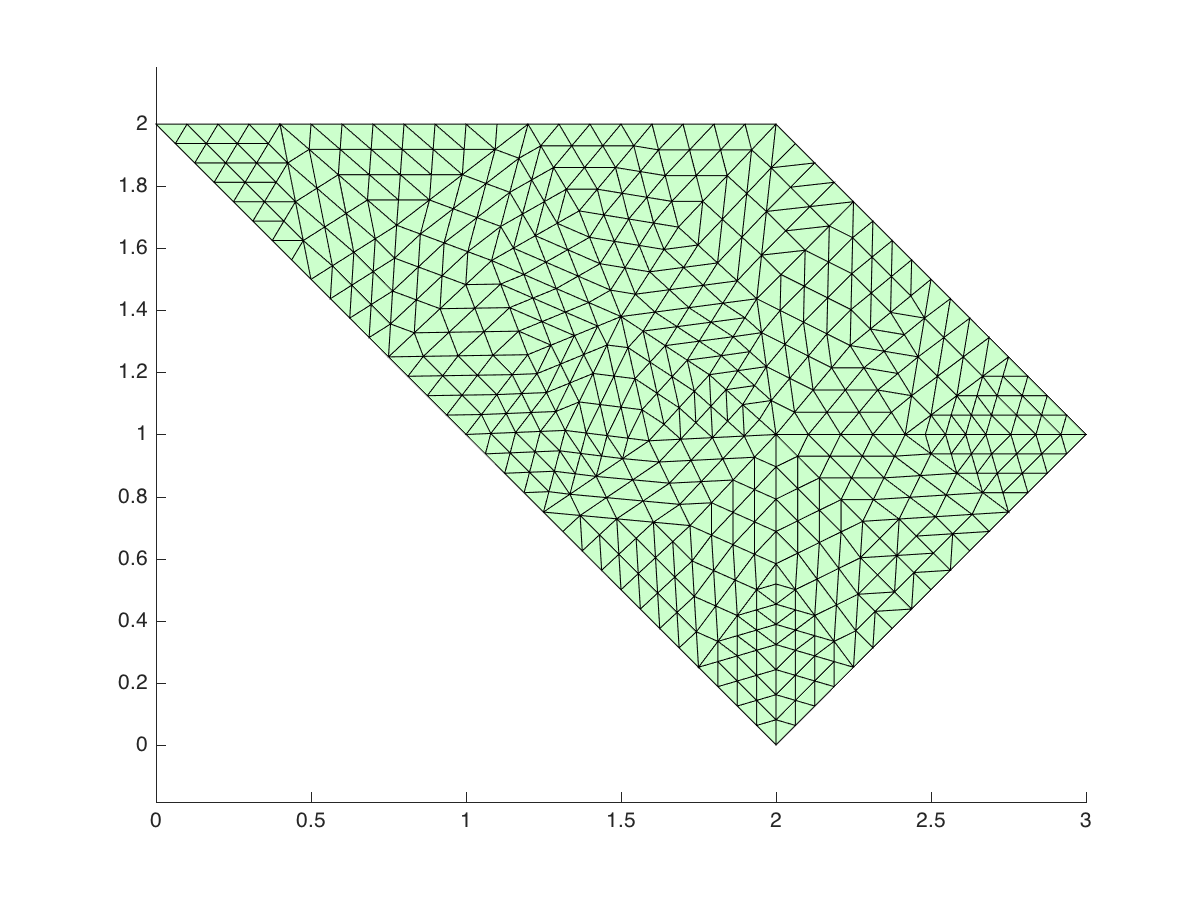
\includegraphics[width=\textwidth]{refine-B2.png}
                \caption{\(n_{ref}=2\)}
        \end{subfigure}%
        \caption{Uniform refinement for different polygon, for \(h_{max}=4\).}
        \label{fig:2}
\end{figure}

Finally, the {\tt boundary\_nodes} function is used to find the indices of all the nodes on the boundary, which is required for later numerical methods such as the finite element method. All of the code used for this problem is included in the Appendix and submitted online. 

\section{Appendix}

\subsection{Question 3 Code}
\subsubsection{{\tt conformal\_map.m}}

This function plots the conformal map in Question 3.

\lstinputlisting[language=Matlab]{conformal_map.m}

\subsection{Question 4 Code}
\subsubsection{{\tt pmesh.m}}

This function is the main function asked for in this problem, and returns the node coordinates, triangulation, and boundary nodes. This function calls several sub-functions that were developed, which are described in the next sections. 

\lstinputlisting[language=Matlab]{pmesh.m}

\subsubsection{{\tt initial\_mesh.m}}

This function places the initial boundary nodes on the boundary according to the requirement that the element side lengths along the boundary be as close as possible to \(h_{max}\), but not exceed this maximum value.

\lstinputlisting[language=Matlab]{initial_mesh.m}

\subsubsection{{\tt delete\_outside.m}}

This function deletes any points that are outside the domain using the {\tt inpolygon} command.

\lstinputlisting[language=Matlab]{delete_outside.m}

\subsubsection{{\tt delete\_outside\_triangles.m}}

This function deletes any triangles that are outside the domain using the {\tt inpolygon} command. A point is placed on each triangle edge at the midpoint, and the {\tt inpolygon} command is used to test whether or not that point is outside the domain. If that point is outside the domain, then the triangle is assumed to be entirely outside the domain, and it is removed from the triangulation.

\lstinputlisting[language=Matlab]{delete_outside_triangles.m}

\subsubsection{{\tt circumcenter.m}}

This function computes the circumcenter of three points. 

\lstinputlisting[language=Matlab]{circumcenter.m}

\subsubsection{{\tt tplot.m}}

This function plots the Delaunay triangulation.

\lstinputlisting[language=Matlab]{tplot.m}

\subsubsection{{\tt boundary\_nodes.m}}

This function returns the indices of nodes on the boundary.

\lstinputlisting[language=Matlab]{boundary_nodes.m}

\end{document}

